\documentclass[tikz,border=6pt]{standalone}
\usepackage{newtxtext,newtxmath}
\usetikzlibrary{arrows.meta,positioning,fit,calc,shapes.geometric}
\usepackage{xcolor}
\definecolor{algred}{RGB}{171,19,30}
\definecolor{softred}{RGB}{249,232,234}
\definecolor{softblue}{RGB}{231,240,250}
\definecolor{softgreen}{RGB}{231,246,237}
\definecolor{softgold}{RGB}{250,244,222}
\definecolor{softgray}{RGB}{242,242,242}
\definecolor{darkgray}{RGB}{55,55,55}
\tikzset{
block/.style={draw,rounded corners=2pt,minimum height=8mm,minimum width=20mm,align=center,font=\small,thick},
state/.style={draw,ellipse,minimum height=7mm,minimum width=15mm,align=center,font=\small},
arrow/.style={-{Latex[length=2mm]},thick},
latent/.style={-{Latex[length=2mm]},thick,dashed,algred},
feedback/.style={-{Latex[length=2mm]},thick,dotted,darkgray},
group/.style={draw,dashed,rounded corners=3pt,inner sep=5pt}
}
\begin{document}
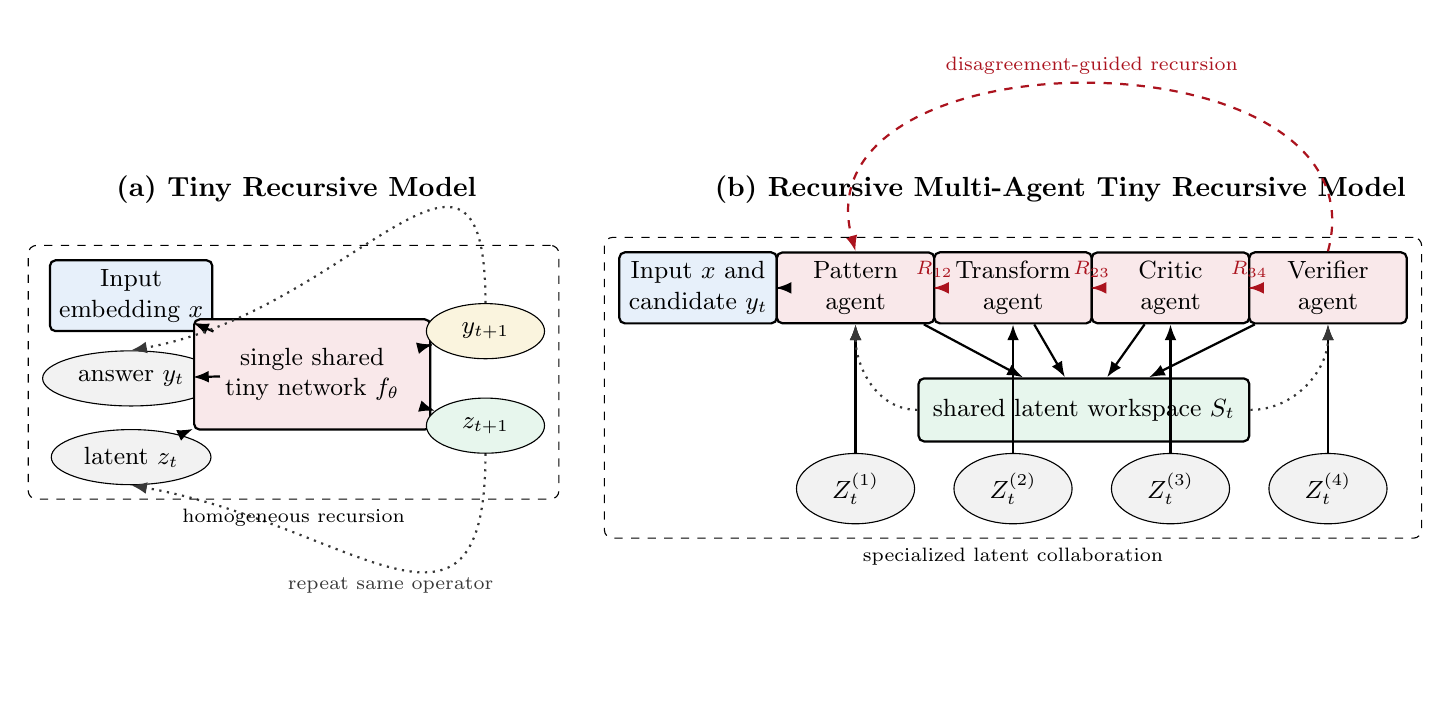
\begin{tikzpicture}[node distance=8mm and 8mm]
\node[font=\bfseries] at (-5.1,2.25) {(a) Tiny Recursive Model};
\node[block,fill=softblue] (x1) at (-7.2,0.9) {Input\\embedding $x$};
\node[state,fill=softgray] (y1) at (-7.2,-0.15) {answer $y_t$};
\node[state,fill=softgray] (z1) at (-7.2,-1.15) {latent $z_t$};
\node[block,fill=softred,minimum width=30mm,minimum height=14mm] (net1) at (-4.9,-0.1) {single shared\\tiny network $f_\theta$};
\node[state,fill=softgreen] (z2) at (-2.7,-0.75) {$z_{t+1}$};
\node[state,fill=softgold] (y2) at (-2.7,0.45) {$y_{t+1}$};
\draw[arrow] (x1) -- (net1);
\draw[arrow] (y1) -- (net1);
\draw[arrow] (z1) -- (net1);
\draw[arrow] (net1) -- (z2);
\draw[arrow] (net1) -- (y2);
\draw[feedback] (z2.south) to[out=-90,in=-10,looseness=1.6] node[below,font=\scriptsize]{repeat same operator} (z1.south);
\draw[feedback] (y2.north) to[out=90,in=10,looseness=1.6] (y1.north);
\node[group,fit=(x1)(y1)(z1)(net1)(z2)(y2),label={[font=\scriptsize]below:homogeneous recursion}] {};

\node[font=\bfseries] at (4.6,2.25) {(b) Recursive Multi-Agent Tiny Recursive Model};
\node[block,fill=softblue] (x2) at (0.0,1.0) {Input $x$ and\\candidate $y_t$};
\node[block,fill=softred] (a1) at (2.0,1.0) {Pattern\\agent};
\node[block,fill=softred] (a2) at (4.0,1.0) {Transform\\agent};
\node[block,fill=softred] (a3) at (6.0,1.0) {Critic\\agent};
\node[block,fill=softred] (a4) at (8.0,1.0) {Verifier\\agent};
\node[block,fill=softgreen,minimum width=42mm] (ws) at (4.9,-0.55) {shared latent workspace $S_t$};
\node[state,fill=softgray] (p1) at (2.0,-1.55) {$Z_t^{(1)}$};
\node[state,fill=softgray] (p2) at (4.0,-1.55) {$Z_t^{(2)}$};
\node[state,fill=softgray] (p3) at (6.0,-1.55) {$Z_t^{(3)}$};
\node[state,fill=softgray] (p4) at (8.0,-1.55) {$Z_t^{(4)}$};
\draw[arrow] (x2) -- (a1);
\draw[latent] (a1) -- node[above,font=\scriptsize]{$R_{12}$} (a2);
\draw[latent] (a2) -- node[above,font=\scriptsize]{$R_{23}$} (a3);
\draw[latent] (a3) -- node[above,font=\scriptsize]{$R_{34}$} (a4);
\foreach \a/\p in {a1/p1,a2/p2,a3/p3,a4/p4}{\draw[arrow] (\p) -- (\a); \draw[arrow] (\a) -- (ws);}
\draw[feedback] (ws.west) to[out=180,in=-90] (a1.south);
\draw[feedback] (ws.east) to[out=0,in=-90] (a4.south);
\draw[latent] (a4.north) to[out=75,in=105,looseness=1.25] node[above,font=\scriptsize]{disagreement-guided recursion} (a1.north);
\node[group,fit=(x2)(a1)(a2)(a3)(a4)(ws)(p1)(p2)(p3)(p4),label={[font=\scriptsize]below:specialized latent collaboration}] {};
\end{tikzpicture}
\end{document}
